\documentclass[12pt, titlepage]{article}

\usepackage{booktabs}
\usepackage{tabularx}
\usepackage{hyperref}
\usepackage{float}
\usepackage{graphicx}
\usepackage[numbers]{natbib}

\usepackage{xcolor}
\usepackage{ulem}

\newcounter{ucnum} %use case number
\newcounter{reqnum} %FRequirement Number
\newcounter{freqnum} %NFRequirement Number

\hypersetup{
    colorlinks,
    citecolor=black,
    filecolor=black,
    linkcolor=red,
    urlcolor=blue
}

\title{\textbf{yoGERT GIS Toolbox}\\ Capstone 4G06\\ Software Requirements Specification}

\author{Team 19,
		\\ Smita Singh, Abeer Alyasiri, Niyatha Rangarajan,\\ Moksha Srinivasan, Nicholas Lobo, Longwei Ye \\\\
		\textbf{Modified Volere Template}
}

\date{\today}

\input{}

\begin{document}

\nocite{*}
\maketitle

\pagenumbering{roman}
\tableofcontents
\listoftables
\listoffigures

\begin{table}[H]
\caption{\bf Revision History}
\begin{tabularx}{\textwidth}{p{3cm}p{2cm}X}
\toprule {\bf Date} & {\bf Version} & {\bf Notes}\\
\midrule
October 5, 2022 & 1.0 & Longwei: Sec 1,8; Moksha: Sec 2.1,8; Smita: Sec 2.1,8; Abeer: Sec 2.2,1.4,1.5; Niyatha: Sec 3; Nicholas: Sec 4,5,6,7 \\
%Date 2 & 1.1 & Notes\\
\bottomrule
\end{tabularx}
\end{table}

\newpage

\pagenumbering{arabic}

%This document describes the requirements for ....  The template for the Software
%Requirements Specification (SRS) is a subset of the Volere
%template~\citep{RobertsonAndRobertson2012}.  If you make further modifications
%to the template, you should explicity state what modifications were made.

\section{Project Drivers}

\subsection{The Purpose of the Project}
Many researchers and companies want to gain information about how people travel, whether that be through the use of personal automobiles, public transit, biking, or even walking. This is because through this data you can derive insights to help inform decisions including but not limited to: public transit design, ad placement, and investment in infrastructure. \\

\noindent When the original GERT toolbox was created, there already existed software to match GPS traces to transportation networks, but the tools suffered had limited usability and functionality \cite{GISBASED}. The GERT toolbox solved this problem by extending functionality, and making the toolbox better suited for multiple input data types. Although the project was a success, it was largely inaccessible due to its reliance on the proprietary and expensive ArcGIS software. \\

\noindent The purpose of the project is to re-engineer the toolbox with a focus on on transferability, modularity, and scalability and remove reliance on any proprietary software so it can be used by a wider audience. 

\subsection{The Stakeholders}
\subsubsection{The Client}
Our main client is Dr. Antonio Paez, a professor in the School of Earth, Environment & Society at McMaster University. 

\subsubsection{The Customers}
Researchers who are interested in matching GPS data to transportation networks in the context of travel episodes and route estimation analysis. Furthermore, companies who are interested in matching GPS data for business analysis and managements. 

\subsubsection{Other Stakeholders}
Developers, testers, and operators of this project.

\subsection{Mandated Constraints}
\begin{itemize}
    \item This project must be completed by the end of April, 2023.
    \item The final product must be able to run on personal laptops and desktops that uses Linux, Windows, and MacOS operating systems with Python pre-installed.
\end{itemize}

\subsection{Naming Conventions and Terminology}
\begin{tabular}{l p{6cm}} 
  \toprule		
  \textbf{symbol} & \textbf{description}\\
  \midrule 
  GPS & Global Positioning Systems\\
  GIS & Geographical Information Systems\\
  GERT & GIS-based episode reconstruction toolkit \\
  Point & location coordinate with time stamp.\\
  Session & Object activity history quantified by GPS points \\
  Episode & Session\\
  Segment & Group of GPS Points combined based on episode attributes.\\
  Trip & GPS points represents an object moving to a different position.\\
  Route & Object path to get from position A to position B\\
  Mode Detection (MD) & Detection of type of transportation being used \\
  Time Use Diary (TUD) & Time Use Diary are records of continuous events and actions through a particular period of time (usually 24 to 48 hours) \\
  Route Choice Analysis (RCA) &  Analyzes route selection from point a to point b\\
  .shp & .shp are geospatial data format files\\
  CSV/.csv & Comma Separated Values is a file type that contains large amounts of data separated by commas. \\
  Potential Activity Locations (PALS) & PALS are potential trip stops \\
  Activity Locations (ALs) & ALs are trip stops \\


  \bottomrule
\end{tabular}\\

\subsection{Relevant Facts and Assumptions}
\begin{itemize}
    \item \sout{As the project is built in python, we assume that the user should be familiar with python.}
    \item Assume users are familiar with CSV files. \textcolor{blue}{ In other words, users should be able to create such files with sufficient information(e.g. latitude and longitude of the points to be dealed with) for the system to generate data.}
    \item Assume users are familiar with map files such as .shp.
\end{itemize}
%As the project is built under python, we assume that the user should be familiar with python.
% User characteristics should go under assumptions.

\newpage
\section{Functional Requirements}

\subsection{The Scope of the Work and the Product}

\subsubsection{The Context of the Work}
The current GERT toolbox is dependent on ARCGIS libraries including arcgisscripting and arcpy. The toolbox currently supports processing GPS files into compatible data types, accurate and fast choice model estimations,  processing millions of GPS data points quickly, extract travel episodes and information on trips, potential activity locations and stops.

\begin{figure}[!h]
	    \begin{center}
    	    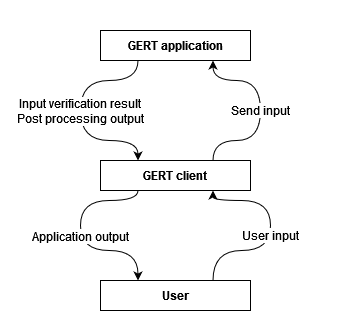
\includegraphics[width=0.75\linewidth]{REV0/SRS/images/gertcontextdiagram.png}
    	    \caption{Context Diagram}
    	    \label{fig: Context Diagram}
    	\end{center}
\end{figure}

\subsubsection{Work Partitioning}
\begin{table}[H]
    \centering
    \begin{tabular}{|p{4cm}|p{4cm}|p{6cm}|}
         \hline
         Event Name & Input and Output & Summary\\
         \hline
         User requests processed gps data & Input: CSV file Output: CSV file & System outputs normalized GPS data\\
         \hline
         User requests GPS episode extraction and mode detection & Input CSV file of gps data, Output: CSV file of of GPS episodes & System outputs episode extraction and mode detection CSV file\\
         \hline
         User requests trip segments based on processed data & Input: CSV file, Output: .shp file & System outputs GPS trip trajectories in a readable format for the user\\
         \hline
         User requests route choice sets & Input: .shp file, Output: .shp file & System outputs route choice sets and allows filtering based on set qualifiers\\
         \hline
         User requests activity locations  & Input: CSV file, Output: .shp file & System outputs activity locations(stops) .shp file\\
         \hline
         User requests route choice analysis variables  & Input: .shp file, Output: .shp file & System outputs the route choice analysis variables along with justification for user perusal \\
         \hline
          User requests activity location identification  & Input: CSV file, .shp file, .shp file, Output: .shp file& System outputs Activity location with Land Use and potential activity locations information in .shp file. \\
         \hline
    \end{tabular}
    \caption{Work Partitioning Diagram\cite{GISBASED}}
    \label{tab:work_partitioning_diagram}
\end{table}

\subsubsection{Product Boundary}
The product boundary diagram was omitted due to redundancy. There are no external services/data sources that the toolbox interacts with. The toolbox may interact with an external open source GIS software, however that is a stretch goal, and should not be factored into initial designs. 

\subsubsection{Product Use Case List}
\begin{figure}[H]
	    \begin{center}
    	    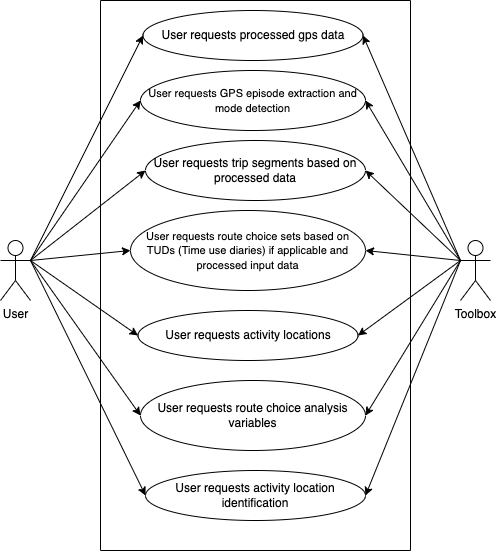
\includegraphics[width=1\linewidth]{REV0/SRS/images/useCaseDiagram.png}
    	    \caption{Use Case Diagram for Toolbox}
    	    \label{fig:Toolbox Use Case Diagram}
    	\end{center}
\end{figure}

\newpage

\subsubsection{Individual Product Use Cases}


\begin{itemize}
    \item[UC\refstepcounter{ucnum}\theucnum
\label{UC_Inputs_1}:] \plt{ \textbf{Name}: Process GPS data\\
        \textbf{Trigger}: User requests processed GPS data\\
        \textbf{Preconditions}: User has a CSV file of unprocessed GPS data \\
        \textbf{Stakeholders}: User, Professor, Geospatial Analyst\\
        \textbf{Actors}: User, Toolbox\\
        \textbf{Outcome}: System outputs a CSV file of normalized GPS data\\}
    \item[UC\refstepcounter{ucnum}\theucnum
\label{UC_Inputs_2}:] \plt{ \textbf{Name}: Episode extraction and mode detection\\
        \textbf{Trigger}: User requests GPS episode extraction and mode detection\\
        \textbf{Preconditions}: User has already requested processed GPS data \\
        \textbf{Stakeholders}: User, Professor, Geospatial Analyst\\
        \textbf{Actors}: User, Toolbox\\
        \textbf{Outcome}: System presents user with a CSV file including all the episodes and mode detection data in a CSV file\\}
    \item[UC\refstepcounter{ucnum}\theucnum
\label{UC_Inputs_3}:] \plt{ \textbf{Name}: Trip segment generation\\
        \textbf{Trigger}: User requests trip segments\\
        \textbf{Preconditions}: System has preprocessed input GPS data, user may optionally input TUD (time use diary) episodes\\
        \textbf{Stakeholders}: User, Professor, Geospatial Analyst\\
        \textbf{Actors}: User, Toolbox\\
        \textbf{Outcome}: .shp file with GPS trip trajectories in a readable format for the user\\}
    \item[UC\refstepcounter{ucnum}\theucnum
\label{UC_Inputs_4}:] \plt{ \textbf{Name}: Route choice set generation\\
        \textbf{Trigger}: User requests route choice sets\\
        \textbf{Preconditions}: System has preprocessed input GPS data and generated trip trajectories file\\
        \textbf{Stakeholders}: User, Professor, Geospatial Analyst\\
        \textbf{Actors}: User, Toolbox\\
        \textbf{Outcome}: .shp file with route choice sets\\}
    \item[UC\refstepcounter{ucnum}\theucnum
\label{UC_Inputs_5}:] \plt{ \textbf{Name}: Activity locations\\
        \textbf{Trigger}: User requests activity locations\\
        \textbf{Preconditions}: System has preprocessed input GPS data and extracted episodes and mode detection CSV file \\
        \textbf{Stakeholders}: User, Professor, Geospatial Analyst\\
        \textbf{Actors}: User, Toolbox\\
        \textbf{Outcome}: System generates .shp file of activity locations (stops)\\}
    \item[UC\refstepcounter{ucnum}\theucnum
\label{UC_Inputs_6}:] \plt{ \textbf{Name}: Route choice analysis variable generation\\
        \textbf{Trigger}: User requests route choice analysis variables\\
        \textbf{Preconditions}: System has preprocessed input GPS data and generated trip trajectories file\\
        \textbf{Stakeholders}: User, Professor, Geospatial Analyst\\
        \textbf{Actors}: User, Toolbox\\
        \textbf{Outcome}: .csv file containing route choice analysis variables and variable justification\\}
    \item[UC\refstepcounter{ucnum}\theucnum
\label{UC_Inputs_7}:] \plt{ \textbf{Name}: Activity location identification\\
        \textbf{Trigger}:User has requested activity location identification\\
        \textbf{Preconditions}: System has preprocessed input GPS data, extracted episodes and mode detection CSV file, and then extracted activity location .shp file, as well as user has inputted land use .shp file potential activity location .shp file \\
        \textbf{Stakeholders}: User, Professor, Geospatial Analyst\\
        \textbf{Actors}: User, Toolbox\\
        \textbf{Outcome}: System outputs a .shp file of activity location with land use and potential activity location information .shp file\\}
\end{itemize}

\subsection{Functional and Data Requirements}
\noindent \begin{itemize}

\item[R\refstepcounter{reqnum}\thereqnum
\label{R_Inputs_1}:] \plt{The system shall allow users to upload GPS data in standard format.}
\begin{itemize}
    \item \textbf{Requirement Type}: Functional
    \item \textbf{Rationale}: The user needs to upload GPS data for processing.
    \item \textbf{Fit Criterion}: The system successfully uploads the file and notifies the user.
    \item \textbf{Priority}: 5
    \item \textbf{Event}: UC1
    \item \textbf{Customer Satisfaction}: 5
    \item \textbf{Customer Dissatisfaction}: 5
    \item \textbf{Conflict}: None
    \item \textbf{Planned Date}: November 14, 2022
\end{itemize}

\item[R\refstepcounter{reqnum}\thereqnum
\label{R_Inputs_1}:] \plt{The system shall process GPS data points.}
\begin{itemize}
    \item \textbf{Requirement Type}: Data
    \item \textbf{Rationale}: System must analysis activity data.
    \item \textbf{Fit Criterion}: The system outputs GPS data points as latitude, longtude, and time variables. 
    \item \textbf{Priority}: 5
    \item \textbf{Event}: UC1
    \item \textbf{Customer Satisfaction}: 5
    \item \textbf{Customer Dissatisfaction}: 5
    \item \textbf{Conflict}: R1.
    \item \textbf{Planned Date}: November 14, 2022
\end{itemize}

\item[R\refstepcounter{reqnum}\thereqnum
\label{R_Inputs_1}:] \plt{The system shall accept TUD data points.}
\begin{itemize}
    \item \textbf{Requirement Type}: Data
    \item \textbf{Rationale}: System must analysis activity data.
    \item \textbf{Fit Criterion}: User successfully upload TUD data in standard format such as CSV. 
    \item \textbf{Priority}: 5
    \item \textbf{Event}: UC3
    \item \textbf{Customer Satisfaction}: 5
    \item \textbf{Customer Dissatisfaction}: 5
    \item \textbf{Conflict}: None
    \item \textbf{Planned Date}: November 14, 2022
\end{itemize}

\item[R\refstepcounter{reqnum}\thereqnum
\label{R_Output_3}:] \plt{The system shall produce output in a standard transferable format.}
\begin{itemize}
    \item \textbf{Requirement Type}: Functional
    \item \textbf{Rationale}: User must read data and re-use output data across multiple applications.
    \item \textbf{Fit Criterion}: System successfully outputs data in standard format such as CSV. 
    \item \textbf{Priority}: 5
    \item \textbf{Event}: UC1-7
    \item \textbf{Customer Satisfaction}: 5
    \item \textbf{Customer Dissatisfaction}: 4
    \item \textbf{Conflict}: None
    \item \textbf{Planned Date}: November 14, 2022
\end{itemize}

\item[R\refstepcounter{reqnum}\thereqnum
\label{R_Inputs_2}:] \plt{The system shall use longitude, latitude, and time variables from GPS data points.}
\begin{itemize}
    \item \textbf{Requirement Type}: Data
    \item \textbf{Rationale}: System must use general variables to make computations and produce analysis.
    \item \textbf{Fit Criterion}: System successfully extracts longitude, latitude, and time information from inputs.
    \item \textbf{Priority}: 5
    \item \textbf{Event}: UC1-7
    \item \textbf{Customer Satisfaction}: 5
    \item \textbf{Customer Dissatisfaction}: 5
    \item \textbf{Conflict}: R2
    \item \textbf{Planned Date}: November 14, 2022
\end{itemize}

\item[R\refstepcounter{reqnum}\thereqnum
\label{R_Outputs_1}:] \plt{The system shall extract episode attributes including speed, duration, direction, distance, change in direction, acceleration, and status points from GPS data points.}
\begin{itemize}
    \item \textbf{Requirement Type}: Functional
    \item \textbf{Rationale}: System must categorize data points to useful information for the user to read.
    \item \textbf{Fit Criterion}: System successfully produce reports of episode attributes. 
    \item \textbf{Priority}: 5
    \item \textbf{Event}: UC2
    \item \textbf{Customer Satisfaction}: 5
    \item \textbf{Customer Dissatisfaction}: 5
    \item \textbf{Conflict}: R5
    \item \textbf{Planned Date}: November 14, 2022
\end{itemize}

\item[R\refstepcounter{reqnum}\thereqnum
\label{R_Inputs_1}:] \plt{The system shall extract episode attributes including duration, distance, and change in trajectory from TUD data points.}
\begin{itemize}
    \item \textbf{Requirement Type}: Functional
    \item \textbf{Rationale}: The system needs to validate  analysis of GPS points.
    \item \textbf{Fit Criterion}: System successfully produce reports of episode attribute.
    \item \textbf{Priority}: 5
    \item \textbf{Event}: UC3
    \item \textbf{Customer Satisfaction}: 5
    \item \textbf{Customer Dissatisfaction}: 4
    \item \textbf{Conflict}: R3
    \item \textbf{Planned Date}: November 14, 2022
\end{itemize}

\item[R\refstepcounter{reqnum}\thereqnum
\label{R_Inputs_1}:] \plt{The system shall classify extracted episode into different types including stop, car, walk, bus, and other travel episodes.}
\begin{itemize}
    \item \textbf{Requirement Type}: Functional
    \item \textbf{Rationale}: User need to understand travel behaviour of objects' episode.
    \item \textbf{Fit Criterion}: System successfully classify predefined examples into correct episode types. 
    \item \textbf{Priority}: 5
    \textbf{Event}: UC2
    \item \textbf{Customer Satisfaction}: 5
    \item \textbf{Customer Dissatisfaction}: 5
    \item \textbf{Conflict}: R6,7
    \item \textbf{Planned Date}: November 14, 2022
\end{itemize}

\item[R\refstepcounter{reqnum}\thereqnum
\label{R_Outputs_2}:] \plt{The system shall decompose episode into output segments of type stop and trip.}
\begin{itemize}
    \item \textbf{Requirement Type}: Functional
    \item \textbf{Rationale}: User need to understand the object's behaviour during a segment.
    \item \textbf{Fit Criterion}: System successfully categorize a moving object in a trip segment and a static object in stop segment
    \item \textbf{Priority}: 5
    \item \textbf{Event}: UC3
    \item \textbf{Customer Satisfaction}: 5
    \item \textbf{Customer Dissatisfaction}: 5
    \item \textbf{Conflict}: R8
    \item \textbf{Planned Date}: November 14, 2022
\end{itemize}

\item[R\refstepcounter{reqnum}\thereqnum
\label{R_Inputs_1}:] \plt{The system shall identify trip trajectory using extracted segments.}
\begin{itemize}
    \item \textbf{Requirement Type}: Functional
    \item \textbf{Rationale}: The system needs trip trajectory for route analysis. 
    \item \textbf{Fit Criterion}: The system successfully identifies the change in the trajectory when the object changes direction. 
    \item \textbf{Priority}: 5
    \item \textbf{Event}: UC3,4
    \item \textbf{Customer Satisfaction}: 5
    \item \textbf{Customer Dissatisfaction}: 5
    \item \textbf{Conflict}: R9
    \item \textbf{Planned Date}: November 14, 2022
\end{itemize}

\item[R\refstepcounter{reqnum}\thereqnum
\label{R_Inputs_1}:] \plt{The system shall identify activity locations based on the episode attributes of the route to the stop point.}
\begin{itemize}
    \item \textbf{Requirement Type}: Functional
    \item \textbf{Rationale}: The system needs location types for land use and road network analysis.
    \item \textbf{Fit Criterion}: The system successfully identify a high activity locations and low activity locations. 
    \item \textbf{Priority}: 5
    \item \textbf{Event}: UC5,7
    \item \textbf{Customer Satisfaction}: 5
    \item \textbf{Customer Dissatisfaction}: 5
    \item \textbf{Conflict}: R6,7
    \item \textbf{Planned Date}: November 14, 2022
\end{itemize}

\item[R\refstepcounter{reqnum}\thereqnum
\label{R_Inputs_1}:] \plt{The system shall generate RCA variables based on trip trajectory.}
\begin{itemize}
    \item \textbf{Requirement Type}: Functional
    \item \textbf{Rationale}: The system needs to define route choice behaviour data set.
    \item \textbf{Fit Criterion}: The system successfully defines variables to describe a route from position A to position B.
    \item \textbf{Priority}: 5
    \item \textbf{Event}: UC4,6
    \item \textbf{Customer Satisfaction}: 5
    \item \textbf{Customer Dissatisfaction}: 4
    \item \textbf{Conflict}: R10
    \item \textbf{Planned Date}: November 14, 2022
\end{itemize}


\item[R\refstepcounter{reqnum}\thereqnum
\label{R_Inputs_1}:] \plt{The system shall store RCA data set.}
\begin{itemize}
    \item \textbf{Requirement Type}: Data
    \item \textbf{Rationale}: The system needs to track the RCA for descriptive route analysis. 
    \item \textbf{Fit Criterion}: System successfully stored multiple instances of RCA variables. 
    \item \textbf{Priority}: 4
    \item \textbf{Event}: UC4,6
    \item \textbf{Customer Satisfaction}: 5
    \item \textbf{Customer Dissatisfaction}: 4
    \item \textbf{Conflict}: R12
    \item \textbf{Planned Date}: November 14, 2022
\end{itemize}

\item[R\refstepcounter{reqnum}\thereqnum
\label{R_Inputs_1}:] \plt{The system shall automate routes from position A to position B based on RCA set.}
\begin{itemize}
    \item \textbf{Requirement Type}: Functional
    \item \textbf{Rationale}: The user wants to request routes from position A to position B.
    \item \textbf{Fit Criterion}: The system produce a mapped route from position A to position B.
    \item \textbf{Priority}: 4
    \item \textbf{Event}: UC6
    \item \textbf{Customer Satisfaction}: 5
    \item \textbf{Customer Dissatisfaction}: 4
    \item \textbf{Conflict}: R13
    \item \textbf{Planned Date}: November 14, 2022
\end{itemize}

\item[R\refstepcounter{reqnum}\thereqnum
\label{R_Inputs_1}:] \plt{The system shall allow users to select options for automated route requests.}
\begin{itemize}
    \item \textbf{Requirement Type}: Functional
    \item \textbf{Rationale}: The user needs the option to customize routes. 
    \item \textbf{Fit Criterion}: The system successfully maps a route with selected options such as shortest distance. 
    \item \textbf{Priority}: 4
    \item \textbf{Event}: UC6
    \item \textbf{Customer Satisfaction}: 4
    \item \textbf{Customer Dissatisfaction}: 4
    \item \textbf{Conflict}: R13
    \item \textbf{Planned Date}: November 14, 2022
\end{itemize}

\item[R\refstepcounter{reqnum}\thereqnum
\label{R_Inputs_1}:] \plt{The system shall store activity location identifications.}
\begin{itemize}
    \item \textbf{Requirement Type}: Data
    \item \textbf{Rationale}: The user needs to search for specific type of activity location.
    \item \textbf{Fit Criterion}: The system successfully stores data and notifies user. 
    \item \textbf{Priority}:4
    \item \textbf{Event}: UC5,7
    \item \textbf{Customer Satisfaction}: 4
    \item \textbf{Customer Dissatisfaction}: 2
    \item \textbf{Conflict}: R11
    \item \textbf{Planned Date}: November 14, 2022
\end{itemize}

\item[R\refstepcounter{reqnum}\thereqnum
\label{R_Inputs_1}:] \plt{The system shall classify RCA patterns by route purpose.}
\begin{itemize}
    \item \textbf{Requirement Type}: Functional
    \item \textbf{Rationale}: The system needs to define trip purpose.
    \item \textbf{Fit Criterion}: The system successfully defines purpose of a route from position A to position B.
    \item \textbf{Priority}: 5
    \item \textbf{Event}: UC4,6
    \item \textbf{Customer Satisfaction}: 5
    \item \textbf{Customer Dissatisfaction}: 4
    \item \textbf{Conflict}: R16,13
    \item \textbf{Planned Date}: November 14, 2022
\end{itemize}

\item[R\refstepcounter{reqnum}\thereqnum
\label{R_Inputs_1}:] \plt{The system shall allows requests for activity location description by filtering.}
\begin{itemize}
    \item \textbf{Requirement Type}: Functional
    \item \textbf{Rationale}: The user needs the options to search for specific type of activity location.
    \item \textbf{Fit Criterion}: The system successfully outputs relevant types of activity locations to what the user requested. 
    \item \textbf{Priority}:4
    \item \textbf{Event}: UC5,7
    \item \textbf{Customer Satisfaction}: 4
    \item \textbf{Customer Dissatisfaction}: 2
    \item \textbf{Conflict}: R16
    \item \textbf{Planned Date}: November 14, 2022
\end{itemize}

\item[R\refstepcounter{reqnum}\thereqnum
\label{R_Inputs_1}:] \plt{The system shall allow users to request trip segments' description for a given GPS data set.}
\begin{itemize}
    \item \textbf{Requirement Type}: Functional
    \item \textbf{Rationale}: The user needs to review intermediate analysis steps. 
    \item \textbf{Fit Criterion}: The system successfully produce trip segment reports. 
    \item \textbf{Priority}: 5
    \item \textbf{Event}: UC3
    \item \textbf{Customer Satisfaction}: 5
    \item \textbf{Customer Dissatisfaction}: 5
    \item \textbf{Conflict}: R9
    \item \textbf{Planned Date}: November 14, 2022
\end{itemize}

\item[R\refstepcounter{reqnum}\thereqnum
\label{R_Inputs_1}:] \plt{The system shall allow users to request episode descriptions of GPS inputs.}
\begin{itemize}
    \item \textbf{Requirement Type}: Functional
    \item \textbf{Rationale}: The user needs to access intermediate details about episode attributes.
    \item \textbf{Fit Criterion}: The system successfully produces a standard output file with the requested details.
    \item \textbf{Priority}: 5
    \item \textbf{Event}: UC2
    \item \textbf{Customer Satisfaction}: 5
    \item \textbf{Customer Dissatisfaction}: 5
    \item \textbf{Conflict}: R6-8
    \item \textbf{Planned Date}: November 14, 2022
\end{itemize}

\end{itemize}


\section{Non-functional Requirements}

\subsection{Look and Feel Requirements}


\subsubsection{Appearance Requirements}
\begin{itemize}
\item[NFR\refstepcounter{freqnum}\thefreqnum
\label{NFR}:] \plt{The system shall be responsive on all devices it is run on. }
\begin{itemize}
    \item \textbf{Rationale}: The system needs to be fully visible and functional for a range of screen widths and heights like an iPad vs a computer.
    \item \textbf{Fit Criterion}: The system's primary functionality as depicted by the user interface is not skewed based on the device it is run on.
    \item \textbf{Priority}: 5
    \item \textbf{Event}: UC1-7 %usecase it relates to
    \item \textbf{Customer Satisfaction}: 5
    \item \textbf{Customer Dissatisfaction}: 5
    \item \textbf{Conflict}: None
    \item \textbf{Planned Date}: November 14, 2022
\end{itemize}
\item[NFR\refstepcounter{freqnum}\thefreqnum
\label{NFR}:] \plt{The system shall display episodes through informative descriptions.}
\begin{itemize}
    \item \textbf{Rationale}:
    \item \textbf{Fit Criterion}: The system is successful if it shows appropriate images of the travel along with appropriate descriptions of its objects on its route.
    \item \textbf{Priority}: 5
    \item \textbf{Event}: UC1 %usecase it relates to
    \item \textbf{Customer Satisfaction}: 5
    \item \textbf{Customer Dissatisfaction}: 5
    \item \textbf{Conflict}: NFR3,4,6; R8
    \item \textbf{Planned Date}: November 14, 2022
\end{itemize}

\subsubsection{Style Requirements}
\item[NFR\refstepcounter{freqnum}\thefreqnum
\label{NFR}:] \plt{The system shall display a modern design templates for its user interface. }
\begin{itemize}
    \item \textbf{Rationale}: The system needs to be catered for different age groups. Considering typical ages 18 onwards, a modern aesthetic would be more appealing.
    \item \textbf{Fit Criterion}:The system is successful if it incorporates modern design frameworks for design of its GUI.
    \item \textbf{Priority}: 5
    \item \textbf{Event}: UC1-7 %usecase it relates to
    \item \textbf{Customer Satisfaction}: 5
    \item \textbf{Customer Dissatisfaction}: 5
    \item \textbf{Conflict}: NFR2,4,6; R8
    \item \textbf{Planned Date}: November 14, 2022
\end{itemize}
\subsection{Usability and Humanity Requirements}

\subsubsection{Ease of Use Requirements}

\item[NFR\refstepcounter{freqnum}\thefreqnum
\label{NFR}:] \plt{The system must be intuitive in terms of its design.}
\begin{itemize}
    \item \textbf{Rationale}: The system must be designed such that its layout of selecting various options (like adding more stops) and position of header descriptions are understandable without a need of additional help.
    \item \textbf{Fit Criterion}: The system is successful if the user is able to interact with the system without customer support.
    \item \textbf{Priority}: 5
    \item \textbf{Event}: UC1-7%usecase it relates to
    \item \textbf{Customer Satisfaction}: 5
    \item \textbf{Customer Dissatisfaction}: 5
    \item \textbf{Conflict}: NFR2,3,6; R8
    \item \textbf{Planned Date}: November 14, 2022
\end{itemize}
\subsubsection{Personalization and Internalization Requirements}

\item[NFR\refstepcounter{freqnum}\thefreqnum
\label{NFR}:] \plt{The system shall provide a feedback option. }
\begin{itemize}
    \item \textbf{Rationale}: The system needs to be updated based on user demand and suggestions.
    \item \textbf{Fit Criterion}: The system is successful if it provides a feedback option for users and protects the anonymity of the user for their feedback.
    \item \textbf{Priority}: 5
    \item \textbf{Event}: UC3-7%usecase it relates to
    \item \textbf{Customer Satisfaction}: 5
    \item \textbf{Customer Dissatisfaction}: 5
    \item \textbf{Conflict}: None
    \item \textbf{Planned Date}: November 14, 2022
\end{itemize}
\subsubsection{Learning Requirements}

\item[NFR\refstepcounter{freqnum}\thefreqnum
\label{NFR}:] \plt{The system's functionality must be easy to understand with inbuilt product descriptions. }
\begin{itemize}
    \item \textbf{Rationale}: The system must be easy to understand for any user on their first use as long as they fall under the appropriate age group of 18 years onwards and follow the instructions presented during use.
    \item \textbf{Fit Criterion}: The system provides information dialogues for complex components of the system.
    \item \textbf{Priority}: 5
    \item \textbf{Event}: UC1-7 %usecase it relates to
    \item \textbf{Customer Satisfaction}: 5
    \item \textbf{Customer Dissatisfaction}: 5
    \item \textbf{Conflict}: NFR2,3,4; R8
    \item \textbf{Planned Date}: November 14, 2022
\end{itemize}
\subsubsection{Understandability and Politeness Requirements}
\item[NFR\refstepcounter{freqnum}\thefreqnum
\label{NFR}:] \plt{The system's must provide a respectful session to the user with salutation greetings.  }
\begin{itemize}
    \item \textbf{Rationale}: In the case of first time users, the system must display more dialogues for showing the spatial arrangements of icons. After more use of the system, the system must greet the on return.
    \item \textbf{Fit Criterion}: The system should display dialogues near icons on first use of the software and allow these icon dialogues to be clickable for future uses. 
    \item \textbf{Priority}: 5
    \item \textbf{Event}: UC1-7%usecase it relates to
    \item \textbf{Customer Satisfaction}: 5
    \item \textbf{Customer Dissatisfaction}: 5
    \item \textbf{Conflict}: None
    \item \textbf{Planned Date}: November 14, 2022
\end{itemize}
\subsubsection{Accessibility Requirements}
\item[NFR\refstepcounter{freqnum}\thefreqnum
\label{NFR}:] \plt{The system's functionality must allow the user to track their progress. }
\begin{itemize}
    \item \textbf{Rationale}: The system must store previously requested GPS points that could be used for future episodes.
    \item \textbf{Fit Criterion}: The system is able to process a request using previously requested GPS data.
    \item \textbf{Priority}: 5
    \item \textbf{Event}: UC3-7%usecase it relates to
    \item \textbf{Customer Satisfaction}: 5
    \item \textbf{Customer Dissatisfaction}: 5
    \item \textbf{Conflict}: None
    \item \textbf{Planned Date}: November 14, 2022
\end{itemize}
\subsection{Performance Requirements}

\subsubsection{Speed and Latency Requirements}
\item[NFR\refstepcounter{freqnum}\thefreqnum
\label{NFR}:] \plt{The system must render the require information within 6000 seconds upon request.}
\begin{itemize}
    \item \textbf{Rationale}: The must process GPS data and display the required episode or stops within a reasonable time.
    \item \textbf{Fit Criterion}: The system takes the GPS data and provides the user with the requested information before 6000 seconds elapses.
    \item \textbf{Priority}: 5
    \item \textbf{Event}: UC7 %usecase it relates to
    \item \textbf{Customer Satisfaction}: 5
    \item \textbf{Customer Dissatisfaction}: 5
    \item \textbf{Conflict}: NFR12,13;R2,4,6,7,8,12
    \item \textbf{Planned Date}: November 14, 2022
\end{itemize}
\subsubsection{Safety Critical Requirements}
\item[NFR\refstepcounter{freqnum}\thefreqnum
\label{NFR}:] \plt{The system must not make the user's location public.}
\begin{itemize}
    \item \textbf{Rationale}: The user's personal information centers around their GPS location. Hence, the system must not make it accessible by the public.
    \item \textbf{Fit Criterion}: The system allows the user to only access their location within their individual session.
    \item \textbf{Priority}: 5
    \item \textbf{Event}: UC2-7%usecase it relates to
    \item \textbf{Customer Satisfaction}: 5
    \item \textbf{Customer Dissatisfaction}: 5
    \item \textbf{Conflict}: None
    \item \textbf{Planned Date}: November 14, 2022
\end{itemize}
\subsubsection{Precision of Accuracy Requirements}
\item[NFR\refstepcounter{freqnum}\thefreqnum
\label{NFR}:] \plt{The system must render the route accurately matching the GPS data points provided.}
\begin{itemize}
    \item \textbf{Rationale}: The route or episode displayed must align with the data points provided to display a relevant and accessible route.
    \item \textbf{Fit Criterion}: The GPS data points requested match the GPS points in the rendered episode.
    \item \textbf{Priority}: 5
    \item \textbf{Event}: UC3-7%usecase it relates to
    \item \textbf{Customer Satisfaction}: 5
    \item \textbf{Customer Dissatisfaction}: 5
    \item \textbf{Conflict}: NFR12; R1-20
    \item \textbf{Planned Date}: November 14, 2022
\end{itemize}
\subsubsection{Robustness or Fault Tolerance Requirements}
N/A
\subsubsection{Capacity Requirements Requirements}
\item[NFR\refstepcounter{freqnum}\thefreqnum
\label{NFR}:] \plt{The system must be able to process 47.3 million points of GPS data.}
\begin{itemize}
    \item \textbf{Rationale}: The route to be generated must be rendered while incorporating precise GPS data. Since, accomodating for more data points would result in an accuarte route, the system should process about a million data points.
    \item \textbf{Fit Criterion}: The system succesfully pases an edge case test with 47.3 million GPS data points requested.
    \item \textbf{Priority}: 5
    \item \textbf{Event}: UC4-7 %usecase it relates to
    \item \textbf{Customer Satisfaction}: 5
    \item \textbf{Customer Dissatisfaction}: 5
    \item \textbf{Conflict}: NFR9; R2,4,6,7,8,12
    \item \textbf{Planned Date}: November 14, 2022
\end{itemize}
\subsubsection{Scalability Requirements}
\item[NFR\refstepcounter{freqnum}\thefreqnum
\label{NFR}:] \plt{The system shall be used by multiple users at a time.}
\begin{itemize}
    \item \textbf{Rationale}: The system will allow multiple users to request for GPS data within their own session at the same time.
    \item \textbf{Fit Criterion}: Two or more users have succesfully rendered their requested GPS data at the same time.
    \item \textbf{Priority}: 5
    \item \textbf{Event}: UC1-7%usecase it relates to
    \item \textbf{Customer Satisfaction}: 5
    \item \textbf{Customer Dissatisfaction}: 5
    \item \textbf{Conflict}: NFR17,18
    \item \textbf{Planned Date}: November 14, 2022
\end{itemize}
\subsubsection{Longevity Requirements}
\item[NFR\refstepcounter{freqnum}\thefreqnum
\label{NFR}:] \plt{The system must be independent of the version of Python.}
\begin{itemize}
    \item \textbf{Rationale}: The system must be upgradable using version updates to the open source software it uses like Python.
    \item \textbf{Fit Criterion}:The system successfully renders the required GPS data independent of the Python version.
    \item \textbf{Priority}: 5
    \item \textbf{Event}: UC1-7%usecase it relates to
    \item \textbf{Customer Satisfaction}: 5
    \item \textbf{Customer Dissatisfaction}: 5
    \item \textbf{Conflict}: None
    \item \textbf{Planned Date}: November 14, 2022
\end{itemize}
\subsection{Operational and Environmental Requirements}

\subsubsection{Expected Physical Environment}
\item[NFR\refstepcounter{freqnum}\thefreqnum
\label{NFR}:] \plt{The system shall be able to run on personal laptops and desktops that uses Linux, Windows, and MacOS operating system with Python pre-installed. }
\begin{itemize}
    \item \textbf{Rationale}: Since it is an open source toolbox, the system only depends on having a valid OS with Python installed.
    \item \textbf{Fit Criterion}: The systems renders the requested GPS data on a valid environment with the stated prerequisites.
    \item \textbf{Priority}: 5
    \item \textbf{Event}: UC1-7%usecase it relates to
    \item \textbf{Customer Satisfaction}: 5
    \item \textbf{Customer Dissatisfaction}: 5
    \item \textbf{Conflict}: NFR16
    \item \textbf{Planned Date}: November 14, 2022
\end{itemize}
\subsubsection{Requirements for Interfacing with Adjacent Systems}
N/A
\subsubsection{Productization Requirements}
N/A
\subsubsection{Release Requirements}
N/A
\subsection{Maintainability and Support Requirements}

\subsubsection{Maintenance Requirements}

\subsubsection{Supportability Requirements}
N/A
\subsubsection{Adaptability Requirements}
\item[NFR\refstepcounter{freqnum}\thefreqnum
\label{NFR}:] \plt{The system must be functional on Linux, Windows, and MacOS operating systems.  }
\begin{itemize}
    \item \textbf{Rationale}: The system must be functionable on a valid OS.
    \item \textbf{Fit Criterion}: The systems renders the requested GPS data on a valid environment with the stated prerequisites.
    \item \textbf{Priority}: 5
    \item \textbf{Event}: UC1-7%usecase it relates to
    \item \textbf{Customer Satisfaction}: 5
    \item \textbf{Customer Dissatisfaction}: 5
    \item \textbf{Conflict}: NFR15
    \item \textbf{Planned Date}: November 14, 2022
\end{itemize}
\subsection{Security Requirements}

\subsubsection{Access Requirements}
\item[NFR\refstepcounter{freqnum}\thefreqnum
\label{NFR}:] \plt{The system must ensure that the user session is password protected. }
\begin{itemize}
    \item \textbf{Rationale}: The user session stores private data of the user and hence, the system must protect it by validating the user through an appropriate password.
    \item \textbf{Fit Criterion}: A user with a password that does not match the stored password can not log into that session.
    \item \textbf{Priority}: 5
    \item \textbf{Event}: UC1-7%usecase it relates to
    \item \textbf{Customer Satisfaction}: 5
    \item \textbf{Customer Dissatisfaction}: 5
    \item \textbf{Conflict}: NFR13,18; R16
    \item \textbf{Planned Date}: November 14, 2022
\end{itemize}
\subsubsection{Integrity Requirements}
\item[NFR\refstepcounter{freqnum}\thefreqnum
\label{NFR}:] \plt{The system shall encyrpt user information. }
\begin{itemize}
    \item \textbf{Rationale}: The system must store information to validate a user for accessing their session. Hence, the system must encrypt such infromation to maintain integrity of their user.
    \item \textbf{Fit Criterion}: The system stores user's personal data using encryption libraries.
    \item \textbf{Priority}: 5
    \item \textbf{Event}: UC1-7%usecase it relates to
    \item \textbf{Customer Satisfaction}: 5
    \item \textbf{Customer Dissatisfaction}: 5
    \item \textbf{Conflict}: NFR13,17
    \item \textbf{Planned Date}: November 14, 2022
\end{itemize}
\subsubsection{Privacy Requirements}
\item[NFR\refstepcounter{freqnum}\thefreqnum
\label{NFR}:] \plt{The system shall not leak sensitive user data. }
\begin{itemize}
    \item \textbf{Rationale}: Since the user's requested locations are stored, the system must only allow valid users to access their session's requested locations.
    \item \textbf{Fit Criterion}: The systems does not allow users from another session to access GPS data outside their session.
    \item \textbf{Priority}: 5
    \item \textbf{Event}: UC1-7%usecase it relates to
    \item \textbf{Customer Satisfaction}: 5
    \item \textbf{Customer Dissatisfaction}: 5
    \item \textbf{Conflict}: NFR13,17,18; R16
    \item \textbf{Planned Date}: November 14, 2022
\end{itemize}

\textcolor{blue}{
\item[NFR\refstepcounter{freqnum}\thefreqnum
\label{NFR}:] \plt{The system shall keep all the data locally. }
\begin{itemize}
    \item \textbf{Rationale}: Since the system is running on user's computer locally, the system must make sure that all the data are kept on the machine only to satisfy the privacy requirement.
    \item \textbf{Fit Criterion}: The system only keeps the executed data on the machine locally.
    \item \textbf{Priority}: 5
    \item \textbf{Event}: UC1-7%usecase it relates to
    \item \textbf{Customer Satisfaction}: 5
    \item \textbf{Customer Dissatisfaction}: 5
    \item \textbf{Conflict}: N/A
    \item \textbf{Planned Date}: November 14, 2022
\end{itemize}
}
\subsubsection{Audit Requirements}
N/A
\subsubsection{Immunity Requirements}
N/A
\subsection{Cultural and Political Requirements}

\subsubsection{Cultural Requirements}
\textcolor{blue}{
\item[NFR\refstepcounter{freqnum}\thefreqnum
\label{NFR}:] \plt{The system shall display proper language. }
\begin{itemize}
    \item \textbf{Rationale}: Since the users of the system have different backgrounds, we must make sure that the words the system displays do not offend them.
    \item \textbf{Fit Criterion}: The words the interface displays to the users are proper, with no violate words.
    \item \textbf{Priority}: 5
    \item \textbf{Event}: UC1-7%usecase it relates to
    \item \textbf{Customer Satisfaction}: 5
    \item \textbf{Customer Dissatisfaction}: 5
    \item \textbf{Conflict}: N/A
    \item \textbf{Planned Date}: November 14, 2022
\end{itemize}
}

\subsubsection{Political Requirements}
N/A
\subsection{Legal Requirements}

\subsubsection{Compliance Requirements}
N/A
\subsubsection{Standards Requirements}
N/A
\subsection{Health and Safety Requirements}
\textcolor{blue}{
\item[NFR\refstepcounter{freqnum}\thefreqnum
\label{NFR}:] \plt{The system shall generate safe or reasonable outputs. }
\begin{itemize}
    \item \textbf{Rationale}: Since some of the data points are lacked of accuracy when the users collect them (e.g. the points in the water or the points that cross the border of the country), the system must ignore those points when processing the data.
    \item \textbf{Fit Criterion}: The system should ignore unreasonable data points when generating the outputs.
    \item \textbf{Priority}: 5
    \item \textbf{Event}: UC1-7%usecase it relates to
    \item \textbf{Customer Satisfaction}: 5
    \item \textbf{Customer Dissatisfaction}: 5
    \item \textbf{Conflict}: N/A
    \item \textbf{Planned Date}: November 14, 2022
\end{itemize}
}

\textcolor{blue}{
\item[NFR\refstepcounter{freqnum}\thefreqnum
\label{NFR}:] \plt{The system must allow users to have access to read and modify the data they've uploaded }
\begin{itemize}
    \item \textbf{Rationale}: This would allow users to edit inputted data and make any necessary changes. If a problem occurs, the user should be able to retrieve their data instead of having to restart the process or software which would be time consuming
    \item \textbf{Fit Criterion}: N/A
    \item \textbf{Priority}: 5
    \item \textbf{Event}: UC1-11%usecase it relates to
    \item \textbf{Customer Satisfaction}: 5
    \item \textbf{Customer Dissatisfaction}: 5
    \item \textbf{Conflict}: N/A
    \item \textbf{Planned Date}: November 14, 2022
\end{itemize}
}

\textcolor{blue}{
\item[NFR\refstepcounter{freqnum}\thefreqnum
\label{NFR}:] \plt{The system shall allow access to all system services and data outputs. }
\begin{itemize}
    \item \textbf{Rationale}: This is the main objective to the application to satisfy user goals. If a problem occurs, the system will be completely ineffective and not workable. 
    \item \textbf{Fit Criterion}: N/A
    \item \textbf{Priority}: 5
    \item \textbf{Event}: UC1-12%usecase it relates to
    \item \textbf{Customer Satisfaction}: 5
    \item \textbf{Customer Dissatisfaction}: 5
    \item \textbf{Conflict}: N/A
    \item \textbf{Planned Date}: November 14, 2022
\end{itemize}
}

\textcolor{blue}{
\item[NFR\refstepcounter{freqnum}\thefreqnum
\label{NFR}:] \plt{The system shall output correct calculated or modified data}
\begin{itemize}
    \item \textbf{Rationale}: The user should not have to question the accuracy of the data outputted. If the data is not accurate or correctly calculated it is contrary to the goal of the system.
    \item \textbf{Fit Criterion}: N/A
    \item \textbf{Priority}: 5
    \item \textbf{Event}: UC1-13%usecase it relates to
    \item \textbf{Customer Satisfaction}: 5
    \item \textbf{Customer Dissatisfaction}: 5
    \item \textbf{Conflict}: N/A
    \item \textbf{Planned Date}: November 14, 2022
\end{itemize}
}

\textcolor{blue}{
\item[NFR\refstepcounter{freqnum}\thefreqnum
\label{NFR}:] \plt{The system will only modify necessary data}
\begin{itemize}
    \item \textbf{Rationale}: The system would be wasting resources and time if any other modification or unnecessary calculations occur. It would also be unethical to use the data in a way that the user is unaware of and has not consented to
    \item \textbf{Fit Criterion}: N/A
    \item \textbf{Priority}: 5
    \item \textbf{Event}: UC1-14%usecase it relates to
    \item \textbf{Customer Satisfaction}: 5
    \item \textbf{Customer Dissatisfaction}: 5
    \item \textbf{Conflict}: N/A
    \item \textbf{Planned Date}: November 14, 2022
\end{itemize}
}

\end{itemize}
\section{Likely Changes}

Automate routes using RCA
\begin{itemize}
\item Using RCA may require extra supporting requirements for functionality and could take more time given. It may not be possible to add this feature into the project.
\end{itemize}
\\
Time Use Diaries
\begin{itemize}
\item Currently users are able to input TUD episodes to generate trip segments. This might require extra supporting requirements in order to accomplish. However, based on time constraints and as it is not one of the main requirements for this project it may not be possible to add this functionality into the final product.
\end{itemize}

\section{Unlikely Changes}

Python as Primary Language
\begin{itemize}
\item Python has many libraries to facilitate mapping and analysing geospatial data which will be integral to creating this software. 
\end{itemize}
\\
GPS Coordinates as Inputs
\begin{itemize}
\item Map matching and extracting episode is dependant on GPS data gathered by the user. 
\end{itemize}
\\
GPS Episodes as Outputs 
\begin{itemize}
\item As the main requirements of the project depends on the usuage of GPS episodes the output is unlikely to change.
\end{itemize}


\section{Traceability Matrix}
\begin{table}[H]
\centering
\scalebox{0.5}{
\begin{tabular}{|c|c|c|c|c|c|c|c|c|c|c|c|c|c|c|c|c|c|c|c|c|}
\hline        
& NFR1 & NFR2 & NFR3 & NFR4 & NFR5 & NFR6 & NFR7& NFR8 & NFR9 & NFR10 & NFR11 & NFR12 & NFR13 & NFR14 & NFR15 & NFR16 & NFR17 & NFR18 & NFR19\\ \hline
R1  & & & &X & &X & & &X &X & &X & & &  & & & &X \\ \hline
R2  & X& & & & & & & X& X& & X& X& X& & & & & & \\ \hline
R3  & & & X& X& X& X& & X& X& X& X& & & & & & & &X \\ \hline
R4  & X& X& X& & & & & & X& & X& & & & & & & & \\ \hline
R5  & & & & & & X& & & & & X& & & X& & & & & \\ \hline
R6  & & X& & & & & & X& X& & X& & & & & & & & \\ \hline
R7  & & X& & & & & & X& X& & X& & & & & & & & \\ \hline
R8  & & X& & X& & X& & X& & & X& & & & & & & & \\ \hline
R9  & & X& & X& & X& & X& & & X& & & & & & & & \\ \hline
R10 & X& X& & & & X& & & X& & X& & & & & & & & \\ \hline
R11 & X& X& & & & X& & & X& & X& & & & & & & & \\ \hline
R12 & X& & & & & & & & X& X& X& & & & & & & & \\ \hline
R13 & X& & & & & & & & X& X& X& & & & & & & & \\ \hline
R14 & X& & & & & & & & X& X& X& & & & & & & & \\ \hline
R15 & X& & X& X& X& X& & & & & & & & & & & & & \\ \hline
R16 & & & & & & & & & X& & & & & & & X& X& X& \\ \hline
R17 & X& & & & & & & & X& X& X& & & & & & & & \\ \hline
R18 & X& X& X& X& & & & X& X& X& & & & & & & & & \\ \hline
R19 & X& X& X& X& & & & X& X& X& & & & & & & & & \\ \hline
R20 & X& X& X& X& & & & & & & & & & & & X& X& X& \\ \hline
\hline
\end{tabular}
}
\caption{Traceability Matrix Showing the Connections Between Functional Requirements and Non Functional Requirements}
\label{Table:trace}
\end{table}

\section{Project Issues}

\subsection{Open Issues}
\begin{itemize}
    \item Understanding the ArcGIS Architecture 
    \item Researching Similar Open Source software to ArcGIS
\end{itemize}

\subsection{Off-the-Shelf Solutions}
The GERT toolbox is the current solution for map matching software. However, it comes with limited functionality and specific data requirements for usage. It is also not open source and expensive to licence. 
\subsection{New Problems}
The software being created is a reworking of the original GERT toolbox and will not interfere with the original toolbox as it is designed separately from it.
\subsection{Tasks}
\begin{itemize}
    \item Hazard Analysis 0
    \item V&V Plan Revision 0
    \item Proof of Concept Demonstration
    \item Design Document Revision 0
    \item Revision 0 Demonstration
    \item V&V Report Revision 0
    \item Final Demonstration
    \item Expo Demonstration
    \item Final Documentation
\end{itemize}
\subsection{Migration to the New Product}
Not applicable to this project. 
\subsection{Risks}
Not applicable to this project. 
\subsection{Costs}
There will be no cost towards making this  toolbox as it is being created completely open source and free from proprietary software.
\subsection{User Documentation and Training}
Documentation will be made using Quarto which is open-source scientific and technical publishing system. This will allow us to put snippets of code within the documentation and will behave as a training manual for users wanting to work with the software. 
\subsection{Waiting Room}
The current plan to for project is a complete re engineering of the GERT toolbox. Once this is completed extra functionality will be added, these include: 
\begin{itemize}
    \item The use of route choice analysis for trip generation 
    \item Using time use diaries for route validation 
\end{itemize}
\subsection{Ideas for Solutions}
At this point in time we are still actively researching different libraries and frameworks to use for this project and they will be added into this section in later revisions of this document. 

\newpage

\section{Appendix}
This section has been added to the Volere template.  This is where you can place
additional information.

\subsection{Symbolic Parameters}

The definition of the requirements will likely call for SYMBOLIC\_CONSTANTS.
Their values are defined in this section for easy maintenance.

\subsection{Reflections}

To successfully complete this project, the team must acquire knowledge related to the content of the toolbox including but not limited to: route choice variables/models, travel episode verification and categorization, trip trajectory generation, GIS software tooling, and understanding various GPS data types. Each member of the team will be responsible for acquiring knowledge on each module of the toolbox. Smita and Moksha will be responsible for route choice variables/models. Longwei will be responsible for trip trajectory generation. Niyatha will be responsible for travel episode verification and categorization. Abeer will be responsible for GIS tooling. Nicholas will be responsible for understanding the GPS data types.\\

\noident To approach this, we meet with domain-specialists including the project's Supervisor, Dr. Paez, past developers of the toolbox, and potential toolbox users. Through interviewing these stakeholders we will learn about the goals of models we are implementing, what is lacking in current tooling, standard GIS software usage, domain specific knowledge regarding trips/routes, and how this information will be used to derive insights. We will also be reading published papers to gain insight on standard GPS data processing algorithms and help discover optimizations for our toolbox.\\

\noindent Another skill our team has to acquire is team management. As a group project, a successful team management strategy will help members complete their tasks more efficiently. We have already established a team communication strategy and methodology for pushing/reviewing content (code, docs, etc.), to complement this, we will routinely schedule retrospectives regarding management strategies to update processes and maximize efficiency. These retrospectives will often consist of identifying productivity blockers, researching better methods, and implementing them into our tooling. \\

\noindent Another skill our team has to acquire is writing and presentation skills. Since every member of the team has different writing experiences, our method of writing varies drastically from person to person. Learning how to write as a team, create formal documentation that is thoroughly consistent with one another will be a challenge. Therefore we will investigate formal writing conventions and ensure that each member of the team is aware and actively uses the predetermined methods. Similarly for the end of the year capstone presentations, the team will have to work together to come up with a method of presentation that will fit all of us as well as be consistent with formal presentation styles. This will require more investigation and practise as a team.\\

\bibliographystyle{IEEEtran}
\bibliography{SRS}

\end{document}
